\documentclass[10pt]{article}
\usepackage[backend=bibtex,style=numeric]{biblatex}
\usepackage{enumitem}
\usepackage{graphicx}
\usepackage{caption}
\usepackage{subcaption}
\usepackage{fullpage}

\addbibresource{refs}

\title{Extracting Application and Menu Events from UI Tutorial Videos}
\author{Daniel Seita \& Andrew Head}

\begin{document}

\maketitle

\begin{abstract}
In this project, we present two main contributions. First, we show that a standard AlexNet neural
network with minimal tweaking can accurately recognize frames belonging to a class of videos.
Second, we present a pipeline for detecting menus within a video frame sequence. We then discuss how
these two stages might be combined to enhance the process of extracting information from videos.
\end{abstract}

\section{Introduction and Motivation}

The proliferation of video tutorials on using different software raises new research questions on
how to improve users' ability to learn from them~\cite{matejka_ambient_2011,
pongnumkul_pause-and-play_2011}.  One strength of video tutorials is that users can directly observe
expert use. Grossman \& Fitzmaurice showed that short, 10-25 second contextually-related videos were
more effective to help users accomplish tasks than traditional text-based
tutorials~\cite{grossman_toolclips_2010}.  Unfortunately, navigation issues could lead to
misunderstanding of content, and users may not be able to keep up with the pace of instruction.
Researchers working with longer, 2-3 minute task-oriented tutorials found that users performed
better with text tutorials than videos because users could not work at the same pace as the
video~\cite{grabler_generating_2009}. In general, research on instructional videos shows a need to
segment videos to emphasize various steps. Our goal in this project is to explore how to segment
existing videos by using computer vision techniques.

By examining pixels, many have succeeded at reverse engineering user interfaces (UIs) and
interactions with purely visual information, independent of underlying application knowledge.  For
instance, Sikuli~\cite{yeh_sikuli_2009} uses computer vision to identify GUI elements from screen
captures by using template matching for small UI elements and voting based on invariant local
features for large elements. Sikuli allows users to search for documentation related to screenshots
of UI elements, and to script GUI tasks using visual cues.

Pause-and-Play extends the template matching approach of Sikuli to detect tool-selection UI events
in compressed, low-resolution video tutorials.  The system takes a tool palette template and tool
icons as input and produces a metadata file of tool changes with timecodes.  With template matching
at multiple resolutions, detection is invariant to recording resolution and some camera
effects~\cite{pongnumkul_pause-and-play_2011}.

% Can cite these but we need more space for actual content: ~\cite{dixon_content_2011}~\cite{dixon_general-purpose_2012}.
Prefab identifies GUI elements with GUI-specific visual features~\cite{dixon_prefab_2010}, which
enables overlay of advanced interactions on existing interfaces.  Prefab identifies interface
elements using two strategies: exact matches of prototype pixels, and models of the background and
pixel differences to identify foreground interface elements. Waken~\cite{banovic_waken_2012}
contributes to this research by discovering cursor shapes, clicking actions, icons, tooltips and
menus, all by examining the difference between frames of UI video.  They do this by making
assumptions about how the image of icons change during hover and press actions.  Detection of the
cursor and icons in later frames is performed by template matching.  We rely on techniques similar
to those in Waken to establish when menus have been activated and menu items selected.


\section{Video Classification}\label{sec:daniel}

As a first step in the information extraction pipeline, we consider the following classification
question: given a video tutorial, what application is it about? We only allow access to the raw
frames, and not metadata such as the video title.  This is an important problem because if we know
the application type of the video tutorial, then we can deploy class-specific extraction procedures,
such as template matching tools based on (for instance) Eclipse videos. Furthermore, if a video
contains multiple applications (e.g., a Microsoft Office video might contain Excel, Powerpont, and
other related products) we might be able to segment the video based on application type, which ties
in to one of our original project goals.

\begin{figure}[t]
\centering
  \begin{minipage}{.4\textwidth}
  \centering
  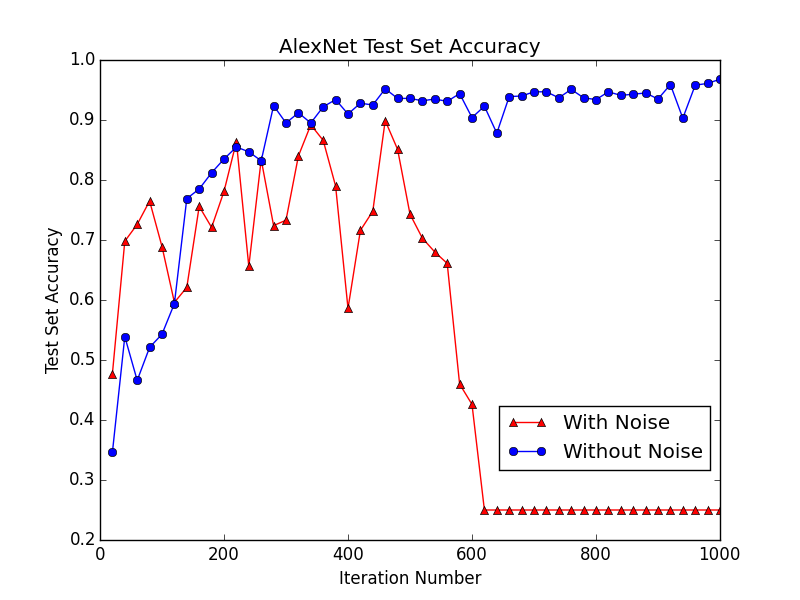
\includegraphics[width=1\linewidth]{AlexNet_Accuracy1000}
  \caption{AlexNet accuracy results of two networks trained on two image datasets.}
  \label{fig:alex_net}
  \end{minipage}\hfill
  \begin{minipage}{.4\textwidth}
  \centering
  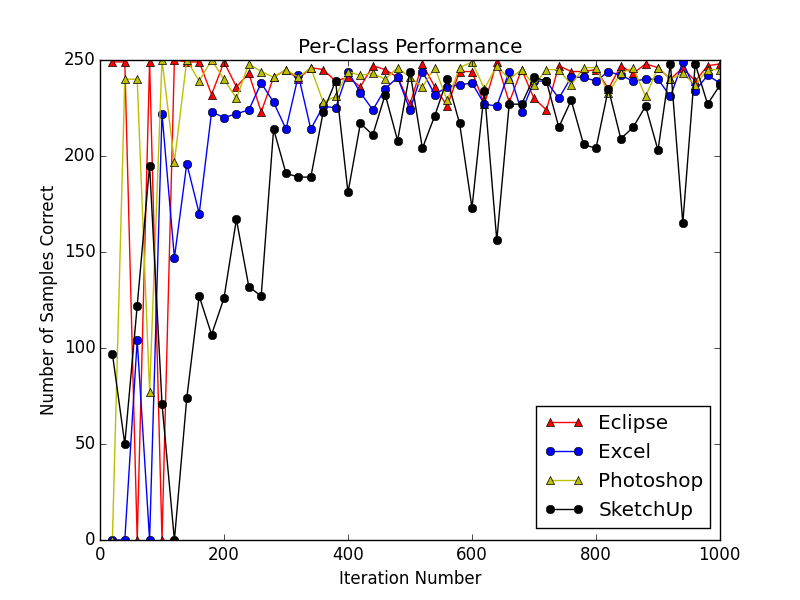
\includegraphics[width=1\linewidth]{PerClassPerformance1000}
  \caption{AlexNet per-class accuracy results for the network trained on ``no noise'' data.}
  \label{fig:per_class}
  \end{minipage}
\end{figure}

To collect training data, we used the \texttt{youtube-dl} software to download YouTube videos into
mp4 format. We restricted our focus to videos about Eclipse, Excel, Photoshop, and SketchUp, and we
extracted from playlists to maintain consistency. Then we used the \texttt{ffmpeg} software to
extract one frame per second from each video, which resulted in a set of 110240 JPG images, roughly
evenly split among the four classes. 

We observed that many of our videos had special introductory and concluding scenes that were of a
different style than the true content of the video. Thus, we created two datasets: one with
\emph{all} the frames, and one with the \emph{first and last ten frames removed} for each video.
Since we had one frame per second, this was equivalent to ``cropping'' each video by ten seconds on
both sides. This cropped dataset, which also included cropped validation and testing frames, was
termed the ``no noise'' data. We randomly divided both datasets into training, validation, and
testing sets, with 52000 training images (13000 per class), 8000 validation images (2000 per class),
and 1000 testing images (250 per class).

To train our network, we used CAFFE's pre-provided AlexNet architecture, but increased the momentum
from 0.9 to 0.99 and decreased the base learning rate from 0.01 to 0.001. We did this because our
batch size of 32 was smaller than the standard 256, so our updates would have been noisier on
average. We ran training for 1000 iterations on both datasets and saved every 20th architecture for
testing purposes.

Figure~\ref{fig:alex_net} shows accuracy results for the two AlexNet networks we trained on the
1000-image test set. The architecture trained on all the data performed inconsistently and its
accuracy eventually leveled off at 25 percent since it always guessed that frames belonged to
SketchUp videos. In contrast, the ``noiseless'' data architecture performed very well, with accuracy
peaking at 96.1 percent after 1000 iterations.

We also investigated per-class accuracy results to see if certain classes of video frames were
harder to learn than others. Figure~\ref{fig:per_class} shows results for the ``no noise'' AlexNet
network. It is clear that SketchUp videos are initially the hardest to learn to identify;
fortunately, by the time we reach 500 iterations, our network can correctly classify the vast
majority of images across all four classes.

We then investigated the 96 filters for the first layer of the AlexNet architecture, each of which
has dimension $55\times 55$. Figures~\ref{fig:filters_all} and~\ref{fig:filters_nonoise} show
visualizations for the two architectures taken after 1000 iterations of training. There are some
interesting patterns, such as straight lines and rough, curved shapes.

\begin{figure}[t]
\centering
  \begin{minipage}{.35\textwidth}
  \centering
  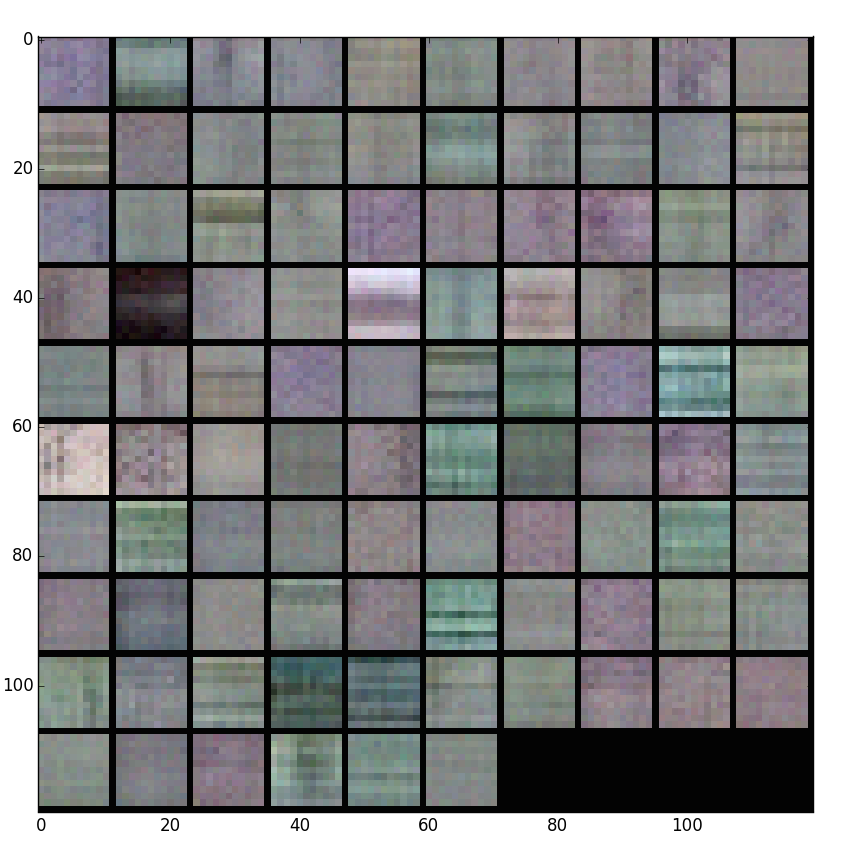
\includegraphics[width=1\linewidth]{Filters_All1000}
  \caption{Visualization of filters from the network trained on all our image data.}
  \label{fig:filters_all}
  \end{minipage}\hfill
  \begin{minipage}{.35\textwidth}
  \centering
  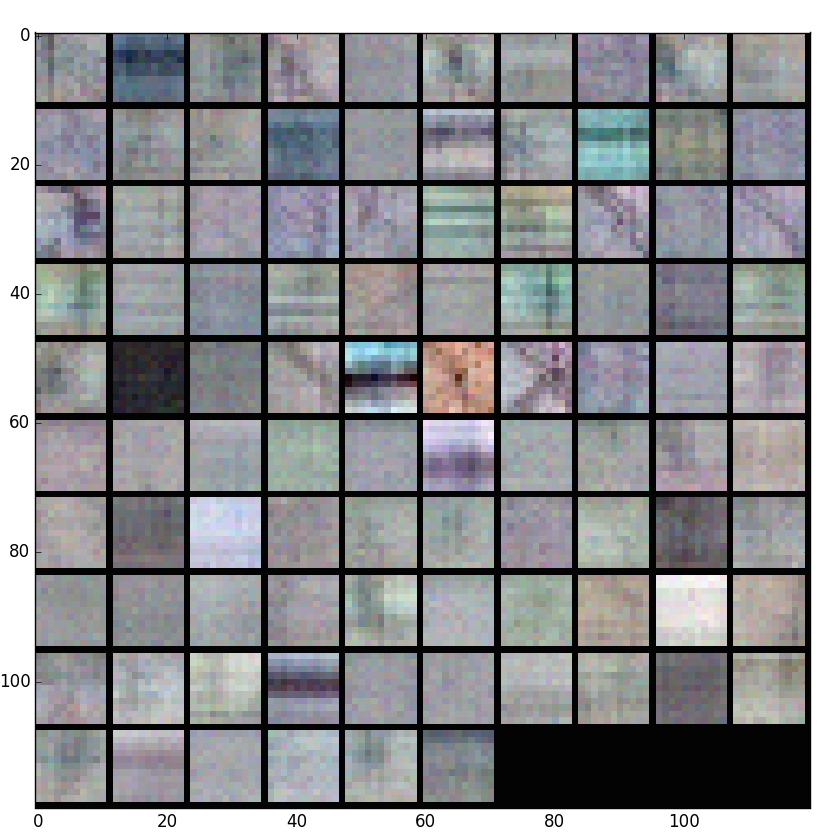
\includegraphics[width=1\linewidth]{Filters_NoNoise1000}
  \caption{Visualization of filters from the network trained on ``no noise'' image data.}
  \label{fig:filters_nonoise}
  \end{minipage}
\end{figure}

Finally, we performed a brief, informal experiment where we applied the (``noiseless'',
1000-iteration) neural network to videos that were not part of our training or testing data. We
chose one video for each of the four classes by searching for tutorials online; we selected the
first video we found that was between 5 and 20 minutes long and not already part of our original
data. We extracted one frame per second and deleted the first and last ten frames.

To describe the output, consider a ``split'' to be $(a,b,c,d)$, which indicates that $a, b, c,$ and
$d$ frames were classified as Eclipse, Excel, Photoshop, and SketchUp, respectively.  The Eclipse
video had $(319,0,79,0)$, the Excel video had $(610,0,71,7)$, the Photoshop had $(1,6,416,69)$, and
the SketchUp had $(9,2,233,804)$. Clearly, for the Eclipse, Photoshop, and SketchUp videos, the
classifier was able to assign the vast majority of frames to the correct class. The Excel output is
unfortunate, but intriguing because our network thought most of the frames belonged to Eclipse
videos. That video we chose was about a newer Excel version (2013) than the one we trained on
(2007).  With a wider variety of Excel frames, we would likely be able to classify that video
correctly.

\section{Locating Menus in a Frame Sequence}\label{andrew}

This will be Andrew's section.

Answer these questions:
\begin{enumerate}[noitemsep]
\item What is our dataset?
\item How did we construct/acquire it?
\item What's its size?
\item (optional) How will we improve it in the future?
\end{enumerate}

Here's a figure of our (edit: Andrew's) pipeline.  \textbf{Andrew: Add figure of pipeline.}

Here we (edit: Andrew) want to touch upon:
\begin{enumerate}[noitemsep]
\item How reliably can we classify UI events?
\item How long does it take for us to process one minute of video?  What are
the practical implications of this?
\item Some images that show recognition results for a few representative
screenshots of user interfaces.
\end{enumerate}


\section{Discussion and Conclusion}

We have described a classifier that can classify video frames, and a pipeline for extracting menus
from videos. Future would would ideally integrate both steps in an overall data mining pipeline by
using class knowledge to develop more specific templates for menu extraction.

\printbibliography

\end{document}
